\documentclass{article}
\usepackage[a4paper, margin=3mm, landscape]{geometry}
\usepackage{multicol}
\usepackage{xcolor}
\usepackage{enumitem}
\usepackage{amsmath}
\usepackage{amsfonts}
\usepackage{listings}
\usepackage{soul}
\usepackage{graphicx}

\pdfinfo{
    /Title (GEC1010.pdf)
    /Creator (TeX)
    /Producer (pdfTeX 1.40.0)
    /Author (Vincent Pang)
    /Subject (GEC1010)
    /Keywords (GEC1010, nus, cheatsheet, pdf)
}

\graphicspath{ {./img/} }

\pagestyle{empty}
\setcounter{secnumdepth}{0}
\setlength{\columnseprule}{0.25pt}

% Redefine section commands to use less space
\makeatletter
\renewcommand{\section}{\@startsection{section}{1}{0mm}%
    {-1ex plus -.5ex minus -.2ex}%
    {0.5ex plus .2ex}%x
{\normalfont\large\bfseries}}
\renewcommand{\subsection}{\@startsection{subsection}{2}{0mm}%
    {-1explus -.5ex minus -.2ex}%
    {0.5ex plus .2ex}%
{\normalfont\normalsize\bfseries}}
\renewcommand{\subsubsection}{\@startsection{subsubsection}{3}{0mm}%
    {-1ex plus -.5ex minus -.2ex}%
    {1ex plus .2ex}%
{\normalfont\small\bfseries}}%
\makeatother

% Adjust spacing for all itemize/enumerate
\setlength{\leftmargini}{0.5cm}
\setlength{\leftmarginii}{0.5cm}
\setlist[itemize,1]{leftmargin=2mm,labelindent=1mm,labelsep=1mm}
\setlist[itemize,2]{leftmargin=2mm,labelindent=1mm,labelsep=1mm}

% Font
\renewcommand{\familydefault}{\sfdefault}

% Define colors for math formulas
\definecolor{myblue}{cmyk}{1,.72,0,.38}
\everymath\expandafter{\the\everymath \color{myblue}}

% Custom command for keywords
\definecolor{highlight}{RGB}{251,243,218}
\newcommand{\keyword}[2][]{\sethlcolor{highlight}\hl{\textbf{#2}} #1 - }
\newcommand{\ilkeyword}[1]{\sethlcolor{highlight}\hl{\textbf{#1}}}

% Define colors and style for code
\definecolor{codegreen}{rgb}{0,0.6,0}
\definecolor{codegray}{rgb}{0.5,0.5,0.5}
\definecolor{codered}{HTML}{CC241D}
\definecolor{backcolor}{rgb}{0.95,0.95,0.95}
\lstdefinestyle{codestyle}{
    backgroundcolor = \color{backcolor},
    commentstyle = \color{codegray},
    keywordstyle = \color{codered},
    stringstyle = \color{codegreen},
    basicstyle = \ttfamily,
    breakatwhitespace = false,
    showstringspaces = false,
    breaklines = true,
    showtabs = false,
    tabsize = 2
}
\lstset{style = codestyle}

% -----------------------------------------------------------------------
\begin{document}
\begin{multicols*}{3}
\footnotesize

% Title box
\begin{center}
    \fbox{
        \parbox{0.8\linewidth}{
            \centering \textcolor{black}{
                {\Large\textbf{GEC1010}} \\
                \normalsize{AY22/23 Sem 2}} \\
                {\footnotesize \textcolor{gray}{github.com/securespider}}
        }
    }
\end{center}
\section{01. Energy}
\subsection{By constant force}
work done by a force == force * displacement
\\$W = FS$
\subsection{Law of conservation of energy}
Energy can neither be created nor destroyed, it can only be transformed from one form to another
\subsection{Kinetic energy}
\keyword{linear motion}{$K=\dfrac{1}{2}mv^2$}\\
\keyword{angular motion}{$\dfrac{1}{2}I\omega^2$}
\begin{itemize}
	\item I = Moment of inertia of object (dependent on mass distribution of object)
	\item $\omega$ = angular velocity of the rotating object
	\begin{itemize}
		\item Rad/second
		\item $v = \omega * radius$
	\end{itemize}
\end{itemize}
\subsection{Gravitational potential energy}
$U = mgh$

\subsection{Power}
Rate of doing work or rate of consumption of energy\\
$P = \dfrac{\triangle W}{\triangle t}$\\
Work done, W, by a system in time t

\subsection{Requirements of an energy system}
\subsubsection{Energy resource}
\begin{itemize}
	\item Clean energy 
	\begin{itemize}
		\item Wind Energy
		\item \keyword{Hydro energy}{Come from river and dams}
		\item Ocean energy{Only refers to energy coming from ocean currents etc}
		\item Solar energy
		\item Biomass
		\item Non-Renewables:
		\item Geothermal
		\item Nuclear
	\end{itemize}
	\item Fossil fuels
	\begin{itemize}
		\item Coal
		\begin{itemize}
			\item Greater carbon content and more impurities - More carbon dioxide and greater air pollution
			\item Solid so difficulty in extraction, transportation and use
			
		\end{itemize}
		\item Natural Gas
		\begin{itemize}
			\item Cleaner alternative 
		\end{itemize}
		\item Oil
	\end{itemize}
\end{itemize}	
Problems
\begin{itemize}
	\item Unsustainable - reserves depleting
	\item Global warming - Enhanced greenhouse effect by earth atmosphere
	\item Greater absorption of long wavelength IR in earth's atmosphere
	\item Rising temperature anomaly from 1980-2000	
	\item Global sea level rising
	\begin{itemize}
		\item Thermal expansion of water
		\item Melting alpine glaciers and ice sheets
	\end{itemize}
	\item Earlier timing of spring events
	\item Poleward and upward shift in plant and animal species
\end{itemize}
Solution:\\
Clean energy
\begin{itemize}
	\item Replace existing supply of fossil fuels
	\item Use energy more efficiently and judiciously minimizing environmental pollution
\end{itemize}
\subsubsection{High power}
\subsubsection{High energy conversion efficiency}
\subsection{Singapore}
Singapore uses LNG primarily (95\%) piped from indonesia and malaysia\\
Switching to solar and biofuels to reduce reliance
\subsubsection{Energy conservation}
\begin{itemize}
	\item Outdoor LED initative
	\item Electric car sharing
\end{itemize}

% -----------------------------------------------------------------------

\section{02. Fundamentals of thermal energy}
$Q=mc\triangle T$
\begin{description}
	\item[Q]{Heat energy supplied}
	\item[m]{mass}
	\item[c]{Specific heat capacity of material}
	\item[T]{temperature change resulting from heat energy}
\end{description}
$Q=mL$
\begin{description}
	\item[Q]{Heat energy supplied}
	\item[m]{mass}
	\item[L]{Specific latent heat of vaporization/fusion}
\end{description}

\subsection{Types}
\begin{itemize}
	\item Conduction
	\begin{itemize}
		\item Dominant in solids
		\item No bulk motion of matter
		\item Heat flows from region of high temperature to region of low temperature
	\end{itemize}
	\item Convection
	\begin{itemize}
		\item Dominant in fluids (liquid and gases)
		\item Works by circulating fluids and thermal expansion properties of materials
		\item Cold fluids sink, warm fluid rise
	\end{itemize}
	\item Radiation
\end{itemize}

\subsection{Stefan Boltzmann Law}
Power of black body radiation\\
$P = \epsilon\sigma T_0^4$
\begin{enumerate}
	\item[P]{Energy absorbed per unit second per unit area via radiation}
	\item[$\epsilon$]{Emissivity of surface(lies between 0-1)}
	\item[$\sigma$]{$5.67*10^{-8}$ = Stefan Boltzmann constant}
\end{enumerate}
\subsection{First law of thermodynamics}
Difference between the heat absorbed Q and the work done W on object is equal to change in internal energy of the thermodynamic system\\
$Q-W=\triangle U$

\subsection{Steam based thermal power plant}
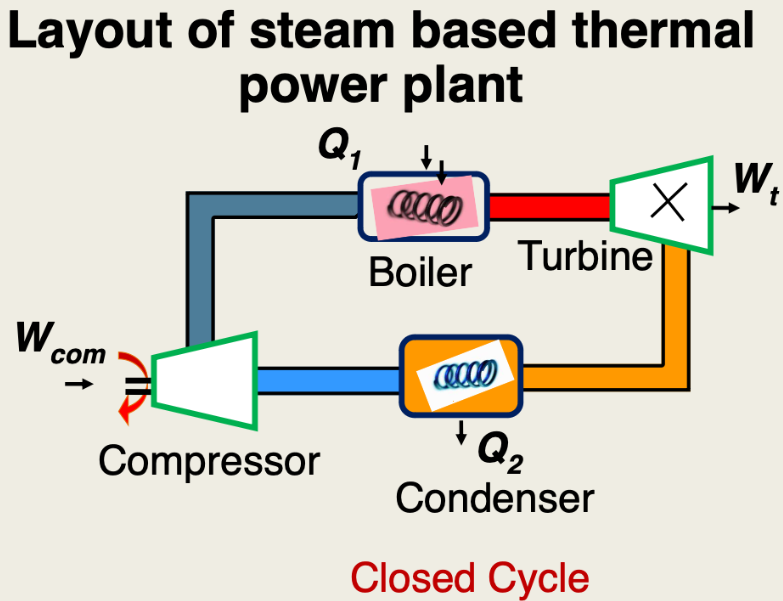
\includegraphics[scale=0.3]{boiler_system}\\
Key stages
\begin{description}
	\item[Compression]{Work done on system to compress cold water to high pressure}
	\item[Boiling]{Heat added to the system to convert cold water into steam}
	\item[Turbine rotation]{Work $W_{t}$ done by the system on turbine blades}
	\item[Condensation]{Heat lost from the system to the environment in converting steam back to cold water}
\end{description}
\begin{itemize}
	\item Working fluid have the same amount of energy U as it had in the beginning of the cycle
%	\item Net work done by the system = $W_t - W_{com}$
	\item Net heat absorbed = $Q_{2} - Q_{2}$
\end{itemize}
Efficiency of cycle is given by \\
$\eta = \dfrac{Net~output~work}{heat~input} = \dfrac{W_{t} - W_{com}}{Q_{1}} = \dfrac{Q_{1}-Q_{2}}{Q_{1}} = 1-\dfrac{Q_{2}}{Q_{1}}$

\subsection{Rankine cycle}
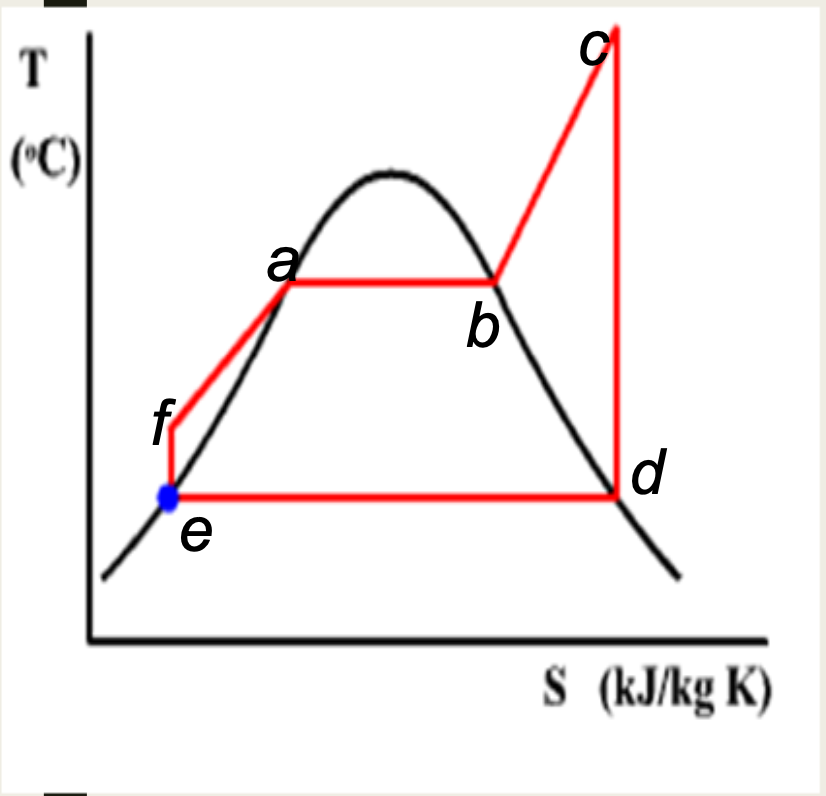
\includegraphics[scale=0.5]{rankine_cycle}\\
Steam power plant energy generation (Temperature - entropy graph)
\begin{itemize}
	\item EF - Compressor increases the pressure of water
	\item FA - Economiser, Water heated at high pressure until it boils
	\item AB - Evaporator, 2 phase mixture of water and steam is heated at constant pressure until all water converted to dry steam
	\item BC - Superheater, Dry steam heated at constant pressure in superheater
	\item CD - Dry steam enter turbine at high pressure and rotate the turbine 
	\item DE - Steam converted to water
	\begin{itemize}
		\item Problem: Unable to completely eliminate the formation of water droplets @ CD
		\item Solution: Reheat the steam at CD to rotate the turbine again
		\item Temperature is raised again, leading to greater efficiency
		\item Achieve 40\% efficiency
		\item Cannot go beyond 650c to prevent metal fatigue
	\end{itemize}
\end{itemize}
\subsection{Brayton cycle}
Use gas instead of water leading to no worry of water droplets and can go higher temperatures


% -----------------------------------------------------------------------
\section{03. Wind energy}
\subsection{How wind forms}
\subsubsection{Dominant}
\begin{itemize}
	\item \keyword{Coriolis Effect}{Sideward component of wind due to earth rotation}
	\item \keyword{Solar radiation}{Warm air rise up in the equator leading to difference in densities}
\end{itemize}

\subsubsection{Other factors}
\begin{itemize}
	\item Ocean
	\begin{itemize}
		\item Water absorbs/releases heat slower than land
		\item Day: Water less hot, sea -> land
		\item Night: Water hotter, land -> sea
	\end{itemize}
	\item Surface friction
	\item Eddy motion
	\item Seasonal effects	
\end{itemize}

\subsection{Power of wind}
$P=\dfrac{1}{2}\rho Au^3$\\
Wind speed affected by height of the turbines
\begin{itemize}
	\item Wind speed rises proportionally to 7th root of altitude
\end{itemize}
\subsection{Wind turbines}
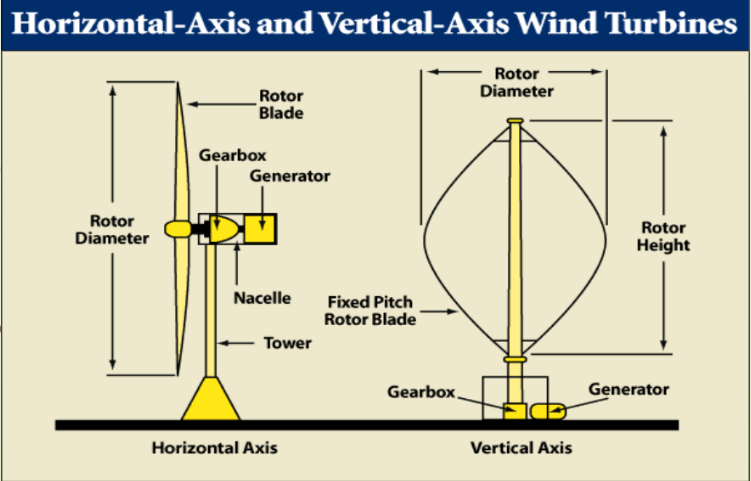
\includegraphics[scale=0.3]{wind-turbine}
\begin{itemize}
	\item \keyword{Yaw control}{Orientates the nacelle in direction of incident wind}
	\begin{itemize}
		\item Note: Better for rotor to face the wind
		\item Less wind shadowing effect
		\item Blades flex less
		\item Less fatigue in the blades
	\end{itemize}
\end{itemize}
\subsection{Forces}
\begin{description}
	\item[Drag]{Net force in direction of wind}
	\item[Lift]{Net force perpendicular to wind}
\end{description}
\subsection{Blades}
Turbines cause turbulence for surrounding blades so cannot have too many blades
\keyword{Tip Speed Ratio (TSR)}{$\dfrac{Speed~of~rotation~of~outer~tip~of~blade}{incident~wind~speed}$}\\
\keyword{Betz limit}{Maximum theoretical efficiency of rotor}\\
\keyword{Capacity factor}{$\dfrac{yield}{rated~power}$}\\
Dependent on wind speed

\subsection{Offshore vs Onshore}
\begin{itemize}
	\item[+] Wind speed is faster offshore
	\item[+] Less obtrusive
	\item[+] Bigger in size
	\item[+] CF higher
	\item[-] Harder to maintain cus in the sea (But easier to build because transportation over water easier)
	\item[-] Might spoil faster due to seawater
\end{itemize}

% -----------------------------------------------------------------------
\section{04a. Solar Power}
Renewable form of energy with $3.9x10^{26}W$\\
Only half reach surface of earth
\subsection{Types of systems}
\begin{itemize}
	\item \keyword{Passive}{Uses no external power}
	\begin{itemize}
		\item Allows fluid heated by the sun to circulate by natural means
	\end{itemize}
	\item \keyword{Active} {Solar heated fluid is circulated by a fan or pump}
\end{itemize}
\subsection{Solar fluid collectors}
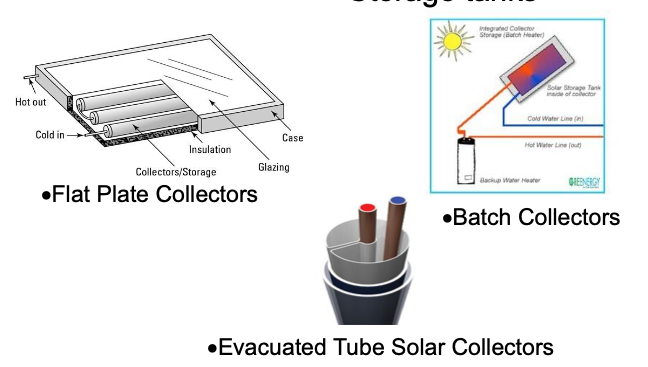
\includegraphics[scale=0.3]{solar-collectors}
\subsection{Passive space heating system}
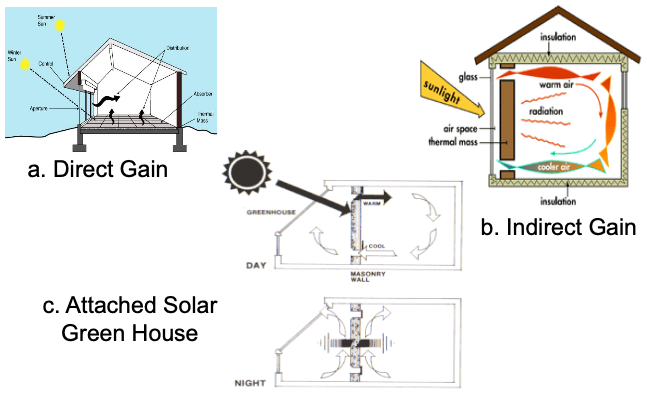
\includegraphics[scale=0.3]{passive-heating}
\subsubsection{Trombe wall}
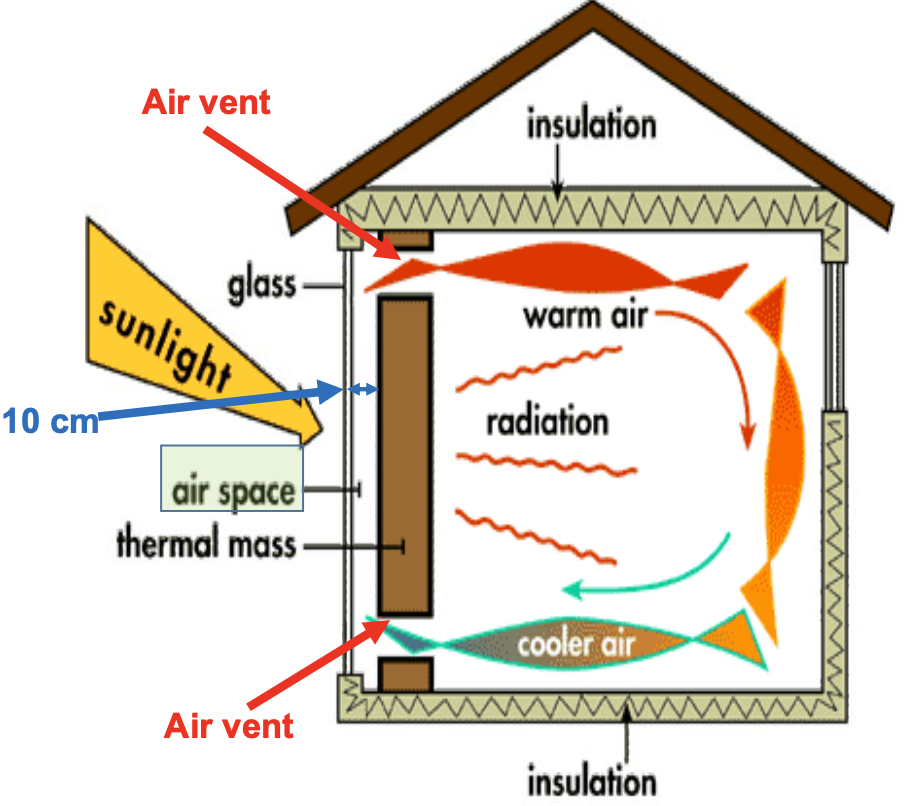
\includegraphics[scale=0.3]{trombe-wall}
\subsection{Principles of passive cooling}
\begin{itemize}
	\item Minimise solar heat gain
	\begin{itemize}
		\item Increase building mass
		\item Increase thermal protection
		\item REflective coating on exposed surface
		\item shading device
		\item Air tightness in building
	\end{itemize}
	\item Remove unwanted heat
	\begin{itemize}
		\item Evaporative cooling
		\item Nocturnal ventilation
		\item Thermo-active ceiling
	\end{itemize}
\end{itemize}
\subsection{Solar power energy}
Using the heat by the sun to drive rankine cycle
\begin{itemize}
	\item using mirrors to focus sun light into a tower to heat molten salt
	\item Run focus pipes surrounded my mirrors to heat the fluid in the pipes to be used to generate heat
\end{itemize}

\subsection{Silicon}

% -----------------------------------------------------------------------
% -----------------------------------------------------------------------
% -----------------------------------------------------------------------

\section{05. Hydro power}
\subsection{Ocean vs River}
River
\begin{enumerate}
	\item Hydroelectricity
\end{enumerate}
Ocean
\begin{enumerate}
	\item Tidal power
	\item Wave power
	\item Ocean thermal
\end{enumerate}
\subsection{Water wheels}
\subsubsection{Water mills}
\begin{itemize}
	\item Ancient application for replacing physical labour
	\item Replaced with water turbines for energy generation
\end{itemize}
Types of water wheels\\
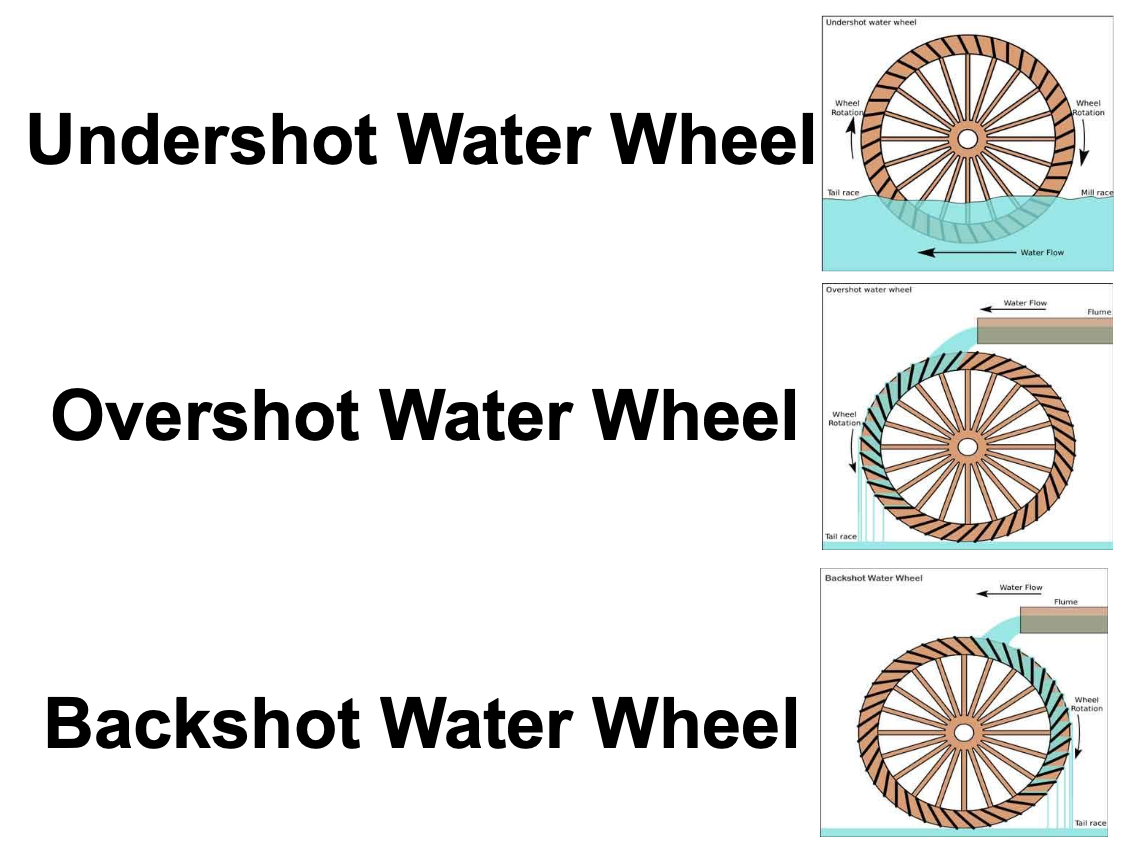
\includegraphics[scale=0.3]{water-wheels}
\begin{itemize}
	\item Undershot
	\begin{itemize}
		\item Vertically mounted with water flowing at the bottom of the wheel
		\item Cheapest and least efficient
	\end{itemize}
	\item Overshot
	\begin{itemize}
		\item Falling water on the top of the wheel in direction of rotation
		\item Use all water flow for power production 
		\item Does not require rapid flow of water
		\item Uses the difference in weight between the 2 sides of the wheel to turn
	\end{itemize}
	\item Backshot
	\begin{itemize}
		\item Introduced behind the apex of the wheel
		\item Water flows opposite the direction of rotation
		\item Continues to function even when water in wheel put rises beyond height of axle
		\item Technique useful for streams that experience extreme seasonal variations in flow
	\end{itemize}
\end{itemize}

\subsection{Types of Hydro Power}
\begin{itemize}
	\item Dam based
	\item Run of the river plants(diversion)
	\item Pumped storage technology
	\item Damless hydro power
\end{itemize}
\subsubsection{Principles of power generation}
Production of electricity by using gravitational force of falling water\\
$P=\eta\rho ghQ$\\
$\eta$ = efficiency, $\rho$ = density of water, Q = Volume of water flowing per second on turbine, h = Vertical distance between turbine and water surface

\end{multicols*}
\end{document}
